
%(BEGIN_QUESTION)
% Copyright 2014, Tony R. Kuphaldt, released under the Creative Commons Attribution License (v 1.0)
% This means you may do almost anything with this work of mine, so long as you give me proper credit

\noindent
{\bf Lab Exercise -- introduction}

\vskip 5pt

Your task is to design and build an analog voltmeter with multiple ranges.  Your project will be centered around a D'Arsonval meter movement, with series-connected ``range'' resistors sized appropriately such that the meter will register precisely full-scale deflection when the expected voltage is applied to the test leads:

$$\includegraphics[width=15.5cm]{i00874x01.eps}$$

The meter movement on its own will be too sensitive to directly connect to any substantial voltage source.  The purpose of each range resistor is to provide just the right amount of electrical resistance that the meter will achieve full-scale deflection when a large, precise voltage is applied to the test jacks.  For example, your meter movement may deflect to full-scale with only a few tenths of a volt applied directly to its terminals, but with the right range resistor connected you will be able to make the needle deflect to full-scale at some larger value such as 10.0 volts or 50.0 volts.

If your meter movement happens to have numbers already written on its face (e.g. 0 to 60), you should exploit these existing labels when choosing your voltage ranges (e.g. 0 to 60 volts, and/or 0 to 6.0 volts).

\vskip 10pt

\filbreak

In designing and constructing this project, you will need to overcome several challenges.  Successful completion of this lab exercise consists of successfully overcoming the following challenges and explaining in detail your solutions to each and every one of them:

\begin{itemize}
\item{} Determining the precise full-scale deflection rating of the meter movement without over-powering it (i.e. causing the needle to {\it slam} or ``peg'' all the way upscale or downscale).
\item{} Determining the precise internal resistance of the meter movement.
\item{} Calculating appropriate range resistor sizes.
\item{} Finding accurate range resistors (or building series/parallel resistor networks to achieve the desired resistance) for each range.
\item{} Identifying ways to make the calibration of your voltmeter adjustable, so that it may be re-calibrated at any time in the future to ensure optimum accuracy.
\item{} How to test your voltmeter to check and demonstrate its accuracy.
\end{itemize}

You are expected to work independently on this project, seeking your own answers and solving problems on your own.  Exachanging ideas with classmates is acceptable, but asking others to solve problems wholesale for you is not.

Your instructor will serve as a resource for you, helping to identify misconceptions and directing you toward helpful resources, as well as overseeing your safety while working in the lab.  It is not your instructor's job, however, to directly answer technical questions that you can and should research for yourself.  One of the over-arching purposes of this lab exercise is to cultivate problem-solving skills and habits.

\underbar{file i00874}
%(END_QUESTION)





%(BEGIN_ANSWER)


%(END_ANSWER)





%(BEGIN_NOTES)


%INDEX% Lab exercise, building an analog voltmeter

%(END_NOTES)

